\documentclass[10pt,twocolumn,letterpaper]{article}

\usepackage{cvpr}
\usepackage{times}
\usepackage{epsfig}
\usepackage{graphicx}
\usepackage{amsmath}
\usepackage{amssymb}


\newcommand{\highlight}[1]{{\color{red}#1}}
% Include other packages here, before hyperref.

% If you comment hyperref and then uncomment it, you should delete
% egpaper.aux before re-running latex.  (Or just hit 'q' on the first latex
% run, let it finish, and you should be clear).
\usepackage[breaklinks=true,bookmarks=false]{hyperref}

\cvprfinalcopy % *** Uncomment this line for the final submission

\def\cvprPaperID{****} % *** Enter the CVPR Paper ID here
\def\httilde{\mbox{\tt\raisebox{-.5ex}{\symbol{126}}}}

% Pages are numbered in submission mode, and unnumbered in camera-ready
%\ifcvprfinal\pagestyle{empty}\fi
\setcounter{page}{1}
\begin{document}

%%%%%%%%% TITLE
\title{Deep Reinforcement Learning for Atari Games}

\author{Liyang Xie \and Xiao Zeng \and Kaixiang Lin\\}
% For a paper whose authors are all at the same institution,
% omit the following lines up until the closing ``}''.
% Additional authors and addresses can be added with ``\and'',
% just like the second author.
% To save space, use either the email address or home page, not both
% \and
% Second Author\\
% Institution2\\
% First line of institution2 address\\
% {\tt\small secondauthor@i2.org}}

\maketitle
%\thispagestyle{empty}


%%%%%%%%% ABSTRACT
\begin{abstract}
%!TEX root = main.tex 
Deep reinforcement learning (DRL) has achieved
unprecedented success in many challenging
domains~\cite{mnih2015human,silver2016mastering}, by combining the power of modeling complex
functions of deep learning and the fairly general-purpose framework of reinforcement learning.
In this project, we \textbf{propose} a new methods that firstly distill the knowledge to a dueling Q-network,
by which the training procedure can be speed up.
Also, we \textbf{implemented} another state-of-arts method--A3C algorithm~\cite{mnih2016asynchronous} as our
baseline.
The extensive experiments have been conducted on OpenAI Gym~\cite{brockman2016openai} to evaluate 
our proposed method and implementations.
% competing state-of-arts such as A3C algorithm~\cite{mnih2016asynchronous}. 
\end{abstract}

%%%%%%%%% BODY TEXT
\section{Introduction}
%!TEX root = main.tex


Deep reinforcement learning has been attracted widely interests from both
industry and academia. The reason is that the combination of deep learning and
reinforcement learning has shown the effectiveness on lots of applications
and more supursingly, the good performances can be achieved without problem-
specific engineering.






OpenAI Gym~\cite{brockman2016openai} is a toolkit for reinforcement learning research. 


%-------------------------------------------------------------------------

\section{Related Work}
%!TEX root = main.tex

The milestone of the deep reinforcement learning is deep Q-learning(DQN)\cite{mnih2013playing}, a variant of Q-learning, proposed by DeepMind. It is the first deep learning model trying to learn control policies with reinforcement learning. In 2015, DeepMind presented an improved version of DQN\cite{mnih2015human}. Their work outperformed previous algorithms and achieved a capability comparable to that of professional human-being.
%

while DQN performs well in fully-observable environments, it achieves poor result in partially observable environments. To address this problem, Hausknecht and Stone\textit{ et al.} \cite{hausknecht2015deep} introduced the Deep Recurrent Q-Networks(DRQN). The idea is to build a recurrent neural network such as LSTM on top of the DQN model.
%

One drawback of DQN is that it needs to aggregate over time to overcome data non-stationarity. To reduce the overhead caused by experience replay, DeepMind \cite{mnih2016asynchronous} proposed a another paradigm for deep reinforcement learning: multiple agents are running in parallel asynchronously on multiple instances of the environment. Using the paradigm makes Q-learning both efficient and compatible with deep neural network at the same time. They named their best method \textit{asynchronous advantage actor-critic} (A3C). Experiments showed that A3C not only achieved better result but also required less computational cost.
%
More recently, AlphaGo\cite{brockman2016openai}, which is also developed by DeepMind, defeated Lee Sedol and became the first 'Artificial Intelligence' who beated 9-dan professional human Go player. Behind the AlphaGo is deep neutral network integrated with reinforcement learning improving the play strategy.
%
One drawback of DQN is that it needs to aggregate over time to overcome data non-stationarity. To reduce the overhead caused by experience replay, DeepMind \cite{mnih2016asynchronous} proposed a very different paradigm for deep reinforcement learning: multiple agents are running in parallel asynchronously on multiple instances of the environment. Using the paradigm makes Q-learning both efficient and compatible with deep neural network at the same time. They named their best method \textit{asynchronous advantage actor-critic} (A3C). Experiments showed that A3C not only achieved better result but also required less computational cost.
%
RDQN sometimes learn unrealistically high action values because it includes a maximization step over estimated action values, which tends to
prefer overestimated to underestimated values. This has been demonstrated in some games in the Atari 2600 domain. The idea of double Q-learning algorithm \cite{van2015deep} not only yields more accurate value estimates, but leads to much higher scores on several games. This demonstrates that the overestimations of DQN indeed lead to poorer policies and that it is beneficial to reduce them.

Other application of reinforcement Learning in designing game includes linear evaluation function-based learning of local shape in the game of Go \cite{silver2007reinforcement} and learning control policies for text-based games \cite{narasimhan2015language}


%-------------------------------------------------------------------------

\section{Methodology}
%!TEX root = main.tex

In this project, we plan to develop and implement a novel deep reinforcement learning algorithm and compete with other methods on OpenAI Gym. Specifically, we will implement DQN and use it as baseline. Based on its performance, we will conduct a series of analysis and try to improve the baseline.
%
DQN adopts a neural network parametrized by $\theta$. The goal is to obtain an optimal estimate of the Q-function by training a model:
\begin{equation*}
\theta = \arg\max_\theta Q(s,a;\theta)
\end{equation*}
where $s$ stands for a state and $a$ denotes the corresponding action. 
The evaluation will be performed on the OpenAI Gym.

The algorithm we used here to beat the baseline is the asynchronous advantage actor-critic (A3C) algorithm that proposed by Volodymyr et al.~\cite{mnih2016asynchronous}. It is a value-based model-free reinforcement learning method. This algorithm maintains a policy $\pi (a_{t}|s_{t};\theta)$ and the estimation of the value function $V(s_{t};\theta_{v})$, where $\theta$ and $\theta_{v}$ are the parameter. These two parameters are learned by the take the gradient of $\log \pi (a_{t}|s_{t};\theta) A(s_{t},a_{t};\theta,\theta_{v})$ with respect to $\theta^{\prime}$. The update of $\pi (a_{t}|s_{t};\theta)$ and $V(s_{t};\theta_{v})$ happens either after every $t_{max}$ actions or when a terminal state is reached. Combine with the idea in deep learning, here we use a convolutional neural network that has one softmax output for the policy $\pi (a_{t}|s_{t};\theta)$ and and
one linear output for the value function $V(s_{t};\theta_{v})$. The algorithm is shown below for completeness.


%-------------------------------------------------------------------------

\section{Experiments}
%!TEX root = main.tex


In this section, we empirically evaluate the effectiveness and the efficiency of the
state-of-arts in deep reinforcement learing on OpenAI gym Atari environment. Note 
that at current stage, we didn't propose any new methods in deep reinforcement learning;
instead our first stage is to learning the most advanced algorithms first using public
available online resources. 


\subsection{Environments}

In order to evaluate the algorithm, we conduct our experiments on Atari environment
provided by OpenAI. The description of Atari environment is as follows:
\begin{quote}
Maximize your score in the Atari 2600 game. In this
environment, the observation is an RGB image of the screen, which is an array
of shape (210, 160, 3) Each action is repeatedly performed for a duration of
kk frames, where kk is uniformly sampled from \{2, 3, 4\}~\cite{brockman2016openai}
\end{quote}

We choose three Atari games as our testing environment, all of which are unsolved environments, 
which means those games don't have a specific reward that you can consider it as the end of game:

\begin{enumerate}
\item Breakout-v0\\
In this game, player control a paddles at the bottom of screen and try to bounce the ball upwards
to hit those bricks as soon and as much as possible, as illustrated in Fig~\ref{fig:A3C_baselines} (a). 

\item Pong-v0\\
In this game, players control a paddles at the right of screen and try to bounce the ball pass the
other player at the left of screen, as illustrated in Fig~\ref{fig:A3C_baselines} (b). 

\item Phoenix-v0
In this game, players control a spaceship by moving it horizontally at the bottom of screen, as 
illustrated in Fig~\ref{fig:A3C_baselines} (c), trying to destroy the enemies by firing upwards 
and avoiding the attack from those enemies. 
\end{enumerate}

\subsection{Baselines}

In this section, we introduce the implementation details of the baselines we used.

% As we introduced in Methodology section, we use two neural network to model policy function
% and value function, respectively. 
The structure of policy network is shown as in Table.\ref{table.cnn_detail}:

\begin{table}[!ht]
	\centering
	\caption{CNN detail}
	\label{table.cnn_detail}
	\begin{tabular}{c|c|c|c}
		\textbf{Type} & \textbf{size} & \textbf{\# filters} & \textbf{activation} \\ \hline
		convolution & $5\times5$ & 32 & Relu \\ 
		max pooling & $2\times2$ &  &  \\
		convolution & $5\times5$ & 32 & Relu \\
		max pooling & $2\times2$ &  &  \\
		convolution & $4\times4$ & 64 & Relu \\
		max pooling & $2\times2$ &  &  \\
		convolution & $3\times3$ & 64 & Relu \\
		fully connected & 512 &  & PRelu \\
		softmax &  &  & 
	\end{tabular}
\end{table}
%\begin{enumerate}
%\item Convolution layer: $(5 \times 5, 32)$ 
%\item Maximum pooling layer: $(2 \times 2) $
%\item Convolution layer: $(5 \times 5, 32)$ 
%\item Maximum pooling layer: $(2 \times 2) $
%\item Convolution layer: $(4 \times 4, 64)$ 
%\item Maximum pooling layer: $(2 \times 2) $
%\item Convolution layer: $(3 \times 3, 64)$ 
%\item Fully connected layer with 512 nodes and PReLU activation function.
%\item Softmax layer to predict the probability over all possible actions.
%\end{enumerate}
We modified the implementation of A3C from \href{https://github.com/ppwwyyxx/tensorpack}{tensorpack} repository.


\subsection{experimental results}




\subsubsection{Policy Gradient}
%!TEX root = main.tex

The results of policy gradient method on CartPole environment is show
in Figure~\ref{fig:pg_cartpole}. Also, a video illustration can be found
in \href{https://gym.openai.com/evaluations/eval_UaXIaMm1QxPGgW45KHtTA#reproducibility}{this link}.
As we can see in both the video and the figure, the game was solved by 
few hundred episodes. This show the effectiveness of policy gradient methods
and we further train a this model in a more complex environment. 

\begin{figure}[h!]
\centering
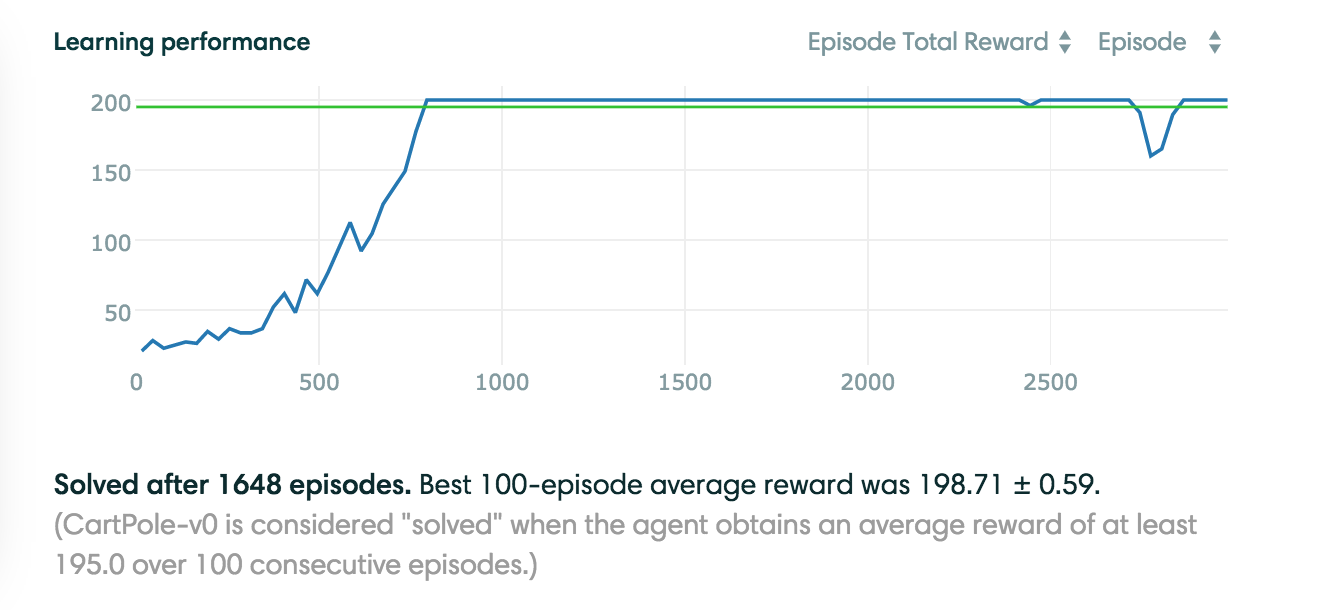
\includegraphics[width=0.49\textwidth]{./fig/pg_cartpole.png} 
\caption{The plot of reward for cartpole game. The x-axis is the number
of episodes it has been trained. The y-axis is the cumulative reward in 
per episode. The higher the better. }
\label{fig:pg_cartpole}
\end{figure}


The performance on Pong game is plot in Figure~\ref{fig:pg_pong} and a video
illustration can be found \href{https://gym.openai.com/evaluations/eval_dODFoXO2S4y5TuUZMX7Nw}{at this link}. As it
shown in the figure, this game requires more than 10000 episodes to get 
a model better than the baseline provided by OpenAI gym. It much more complicated
than the CartPole, since the state and action space is more complex than 
that. The structure of this policy is a single hidden layer with eight
hidden nodes fully connected network and it works. It may perform
better if we use a convolutional network to replace this one, but compared 
the results in dueling DQN, it seems the algorithms of reinforcement learning
itself is more important, other than the specific network architecture. 

\begin{figure}[h!]
\centering
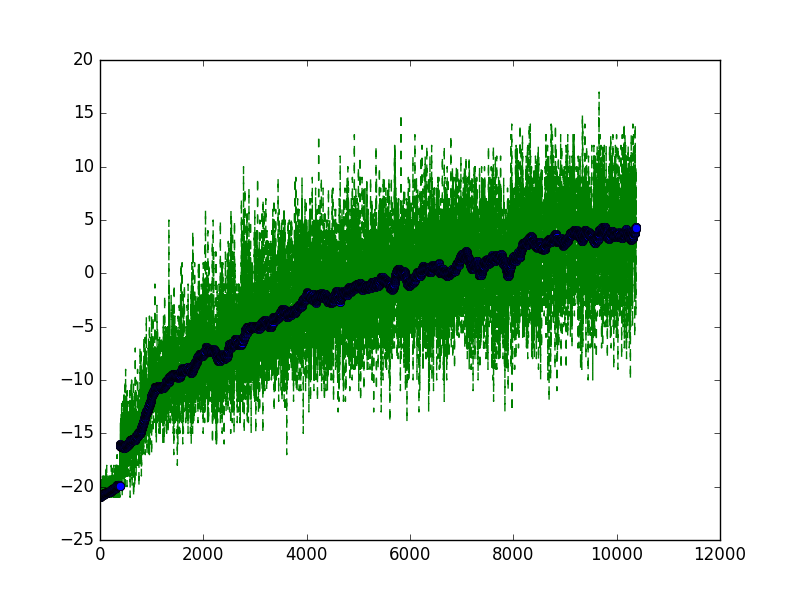
\includegraphics[width=0.49\textwidth]{./fig/pg_pong_rewardsplot.png} 
\caption{The plot of reward for pong game. The x-axis is the number
of episodes it has been trained. The y-axis is the cumulative reward in 
per episode. The higher the better. }
\label{fig:pg_pong}
\end{figure}




\subsubsection{Asynchronous advantage actor-critic}
The experimental results are illustrated in the Fig~\ref{fig:A3C_baselines}. Please also
see the video animation by clicking the captions under each figures. 
% The results are acquired by a pre-trained model and then follow the A3C models,

\begin{figure}[h!]
\centering
\begin{tabular}{c}
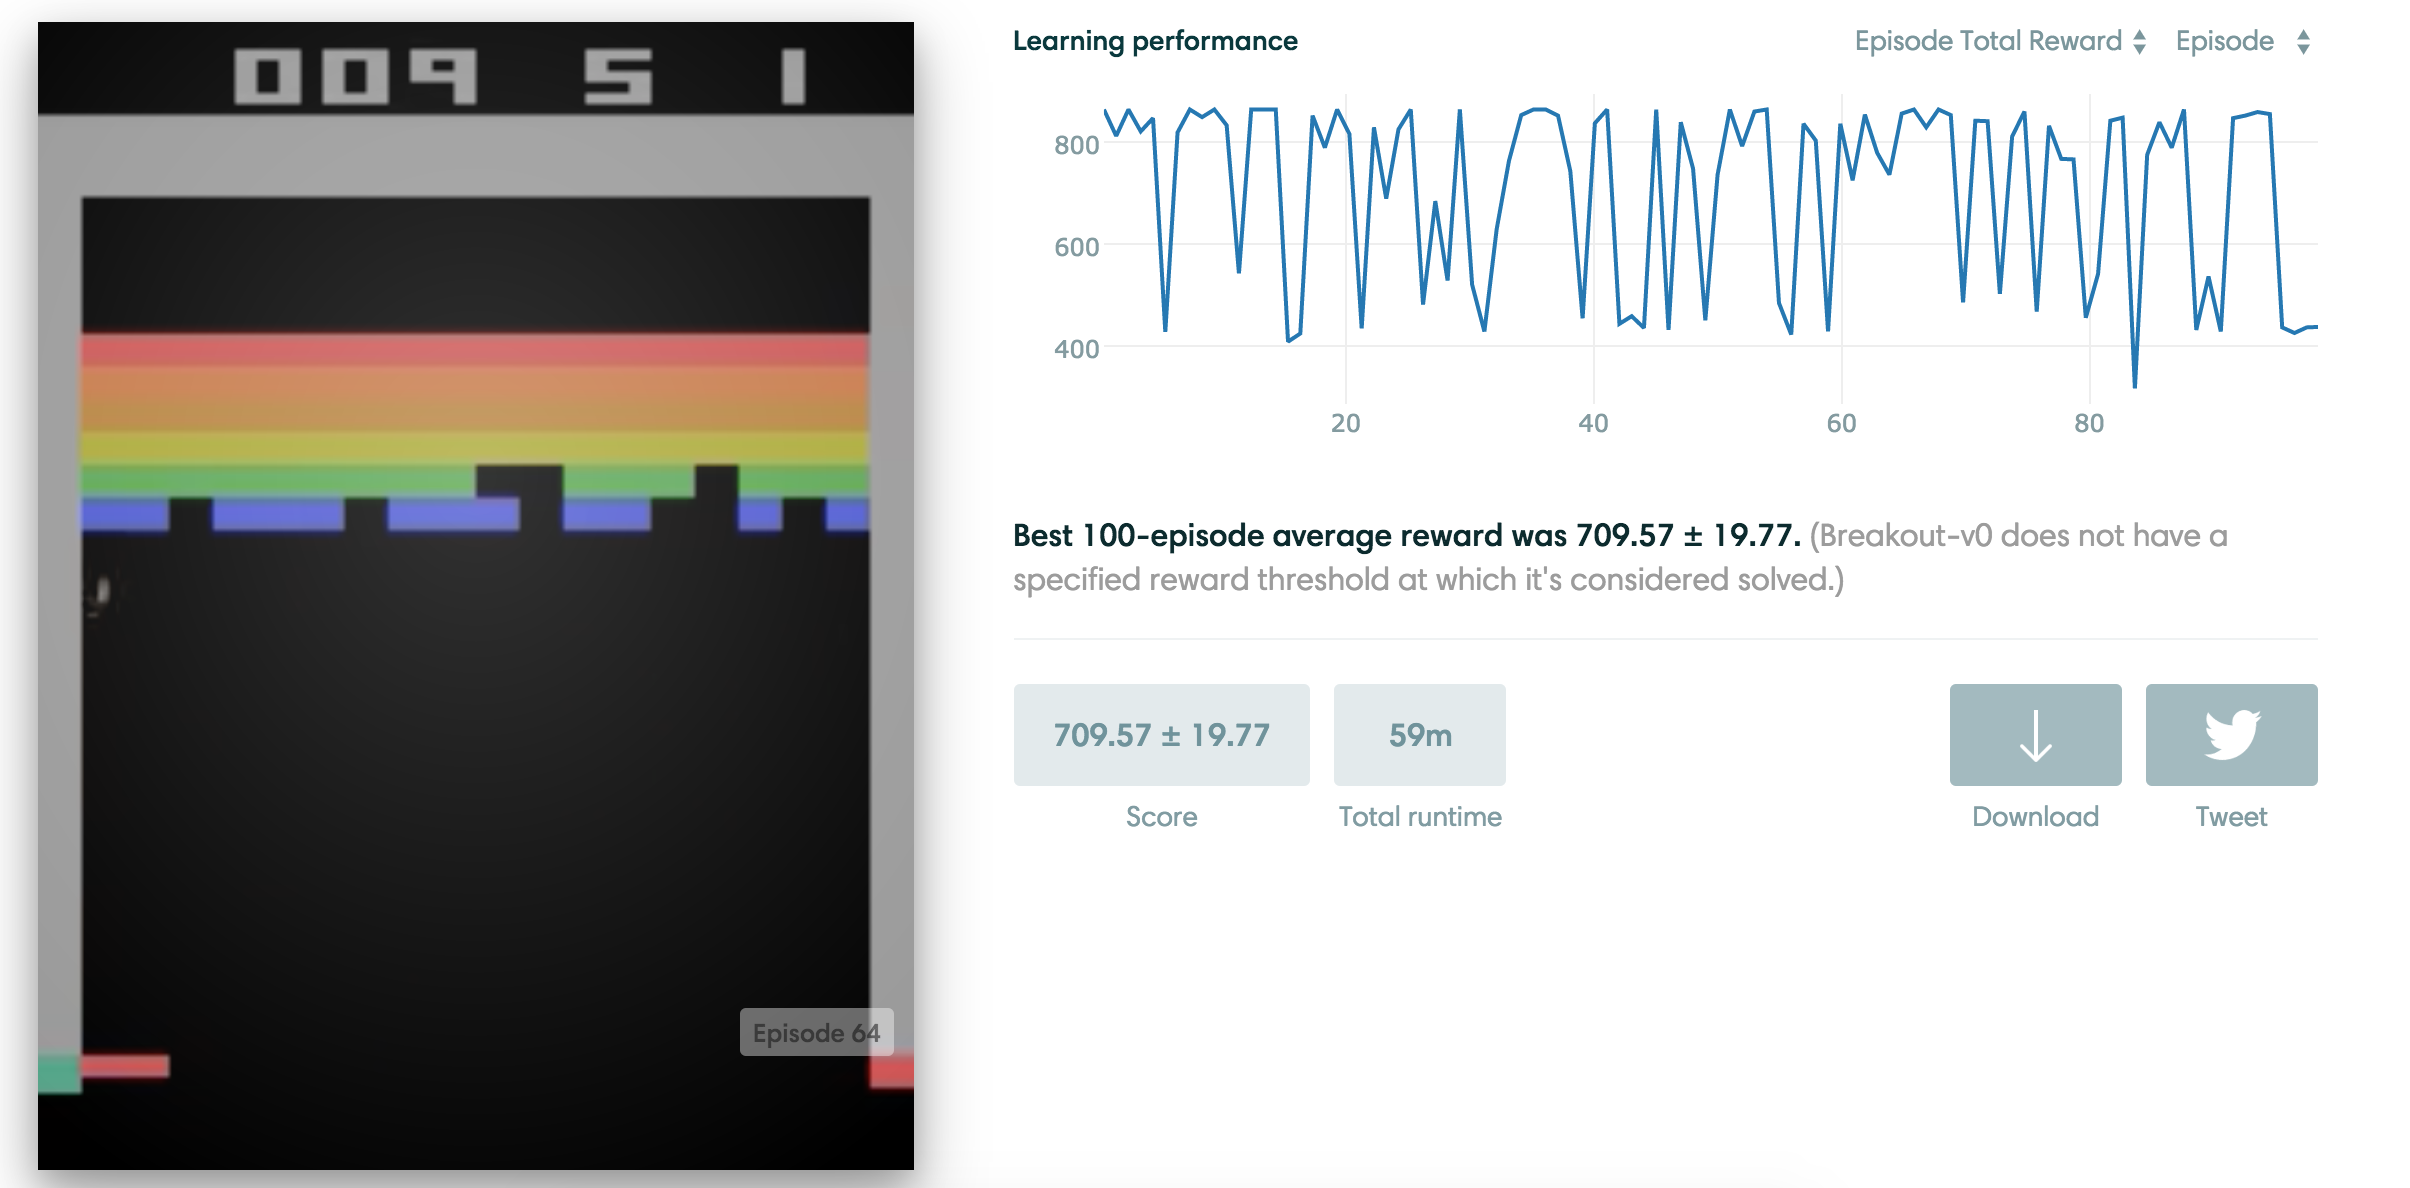
\includegraphics[width=0.49\textwidth]{./fig/A3C_Breakout-v0.png} \\
(a) \href{https://gym.openai.com/evaluations/eval_i9E40nAQuOTiSa0bxYBA#reproducibility}{Breakout-v0} \\
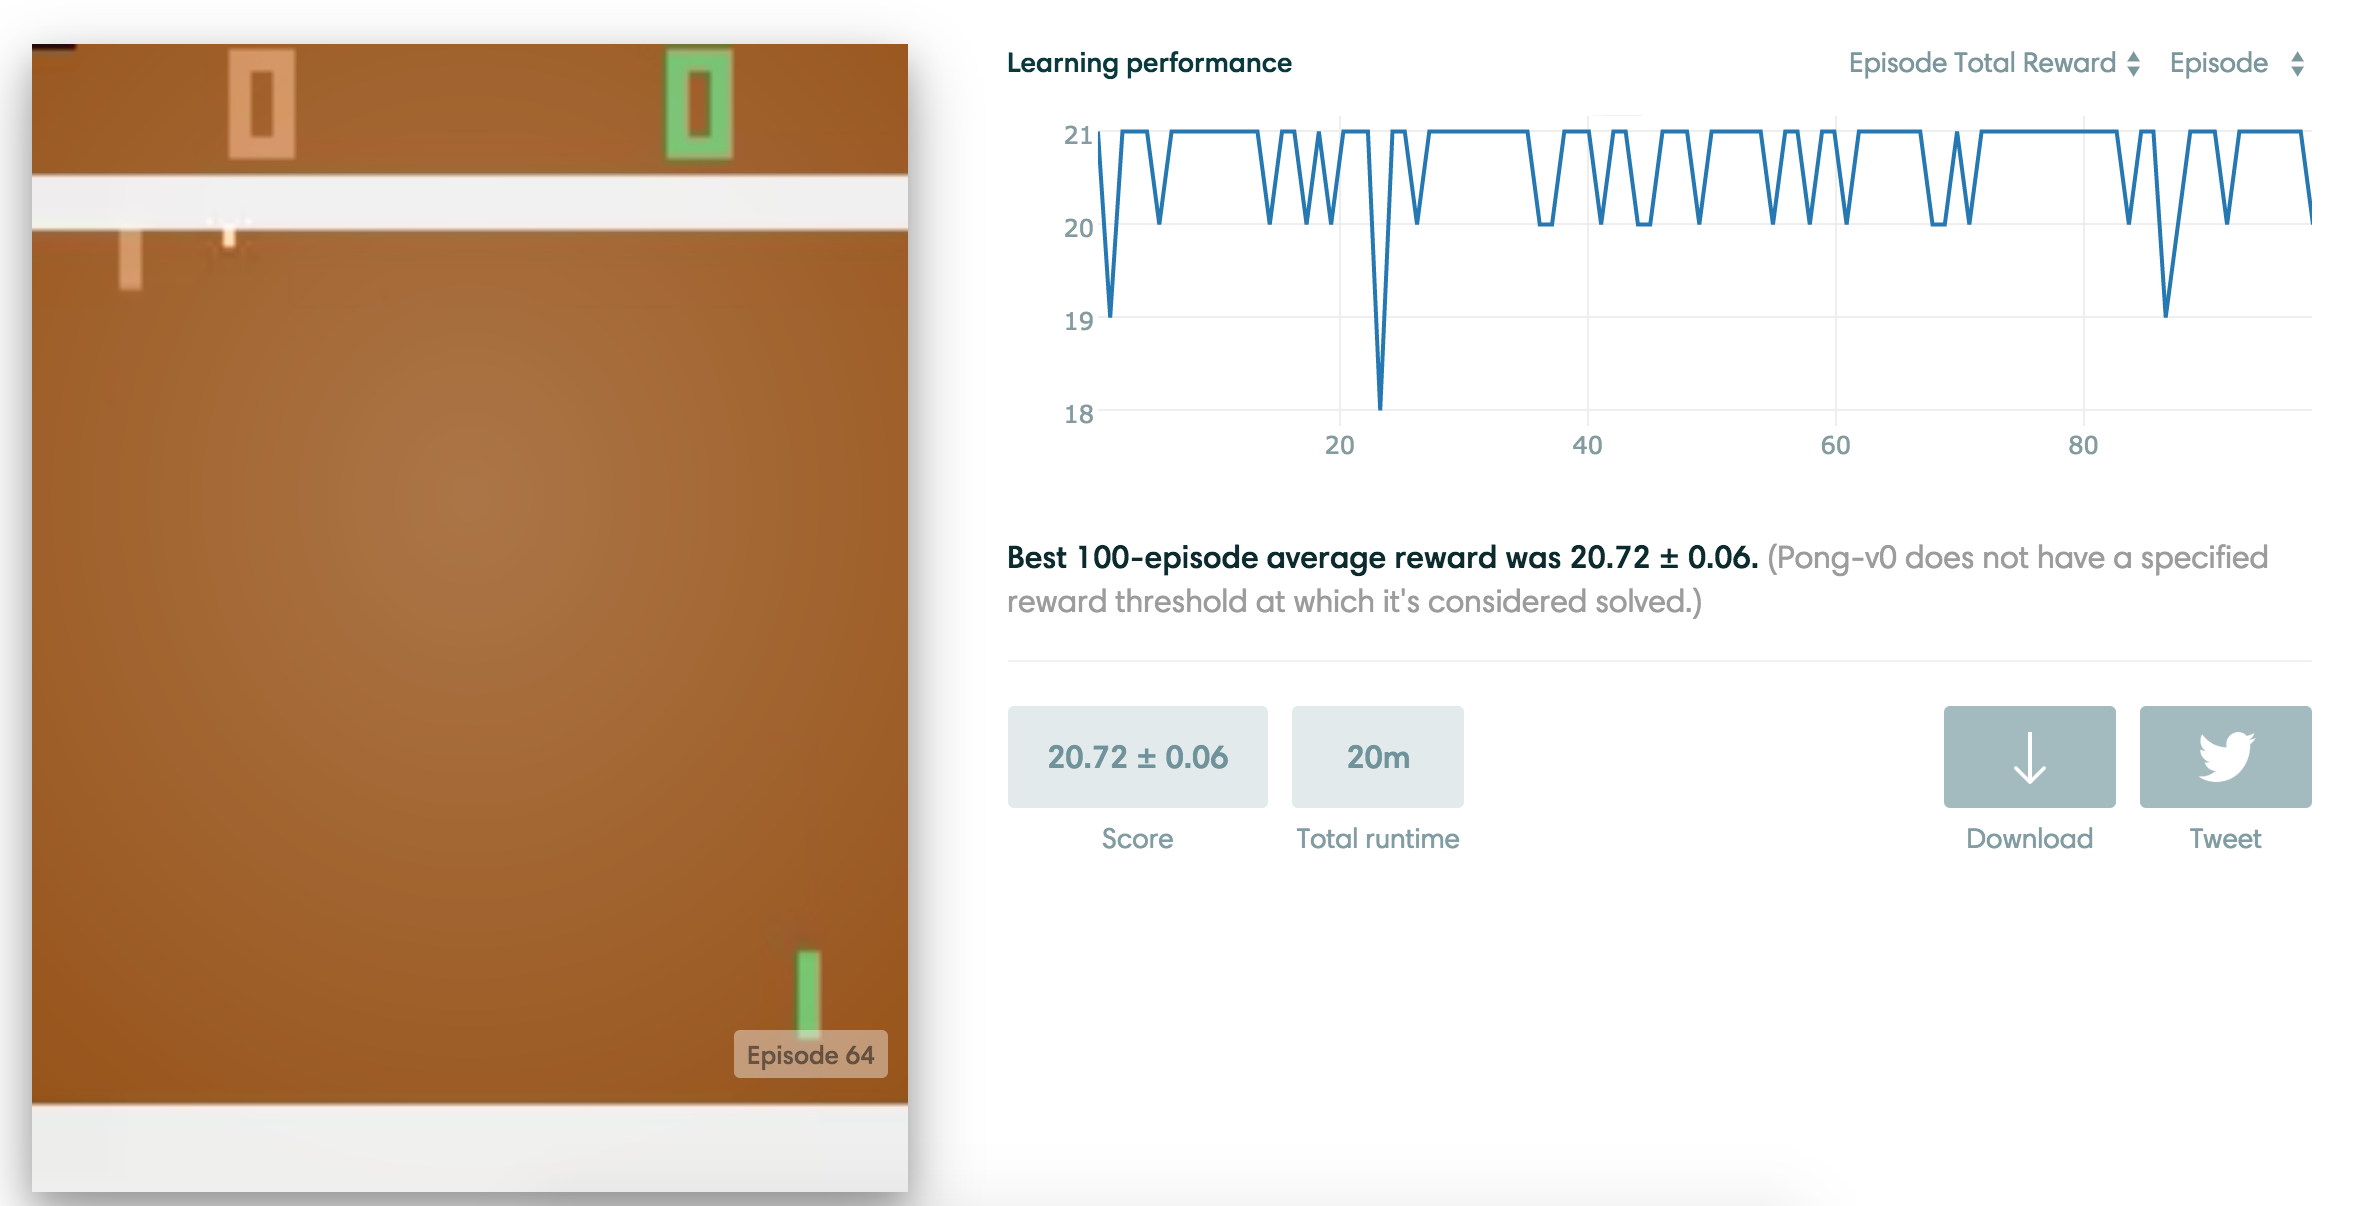
\includegraphics[width=0.49\textwidth]{./fig/A3C_Pong-v0.png} \\
(b) \href{https://gym.openai.com/evaluations/eval_mvXuxP13SSacO01UIhsg#reproducibility}{Pong-v0} \\
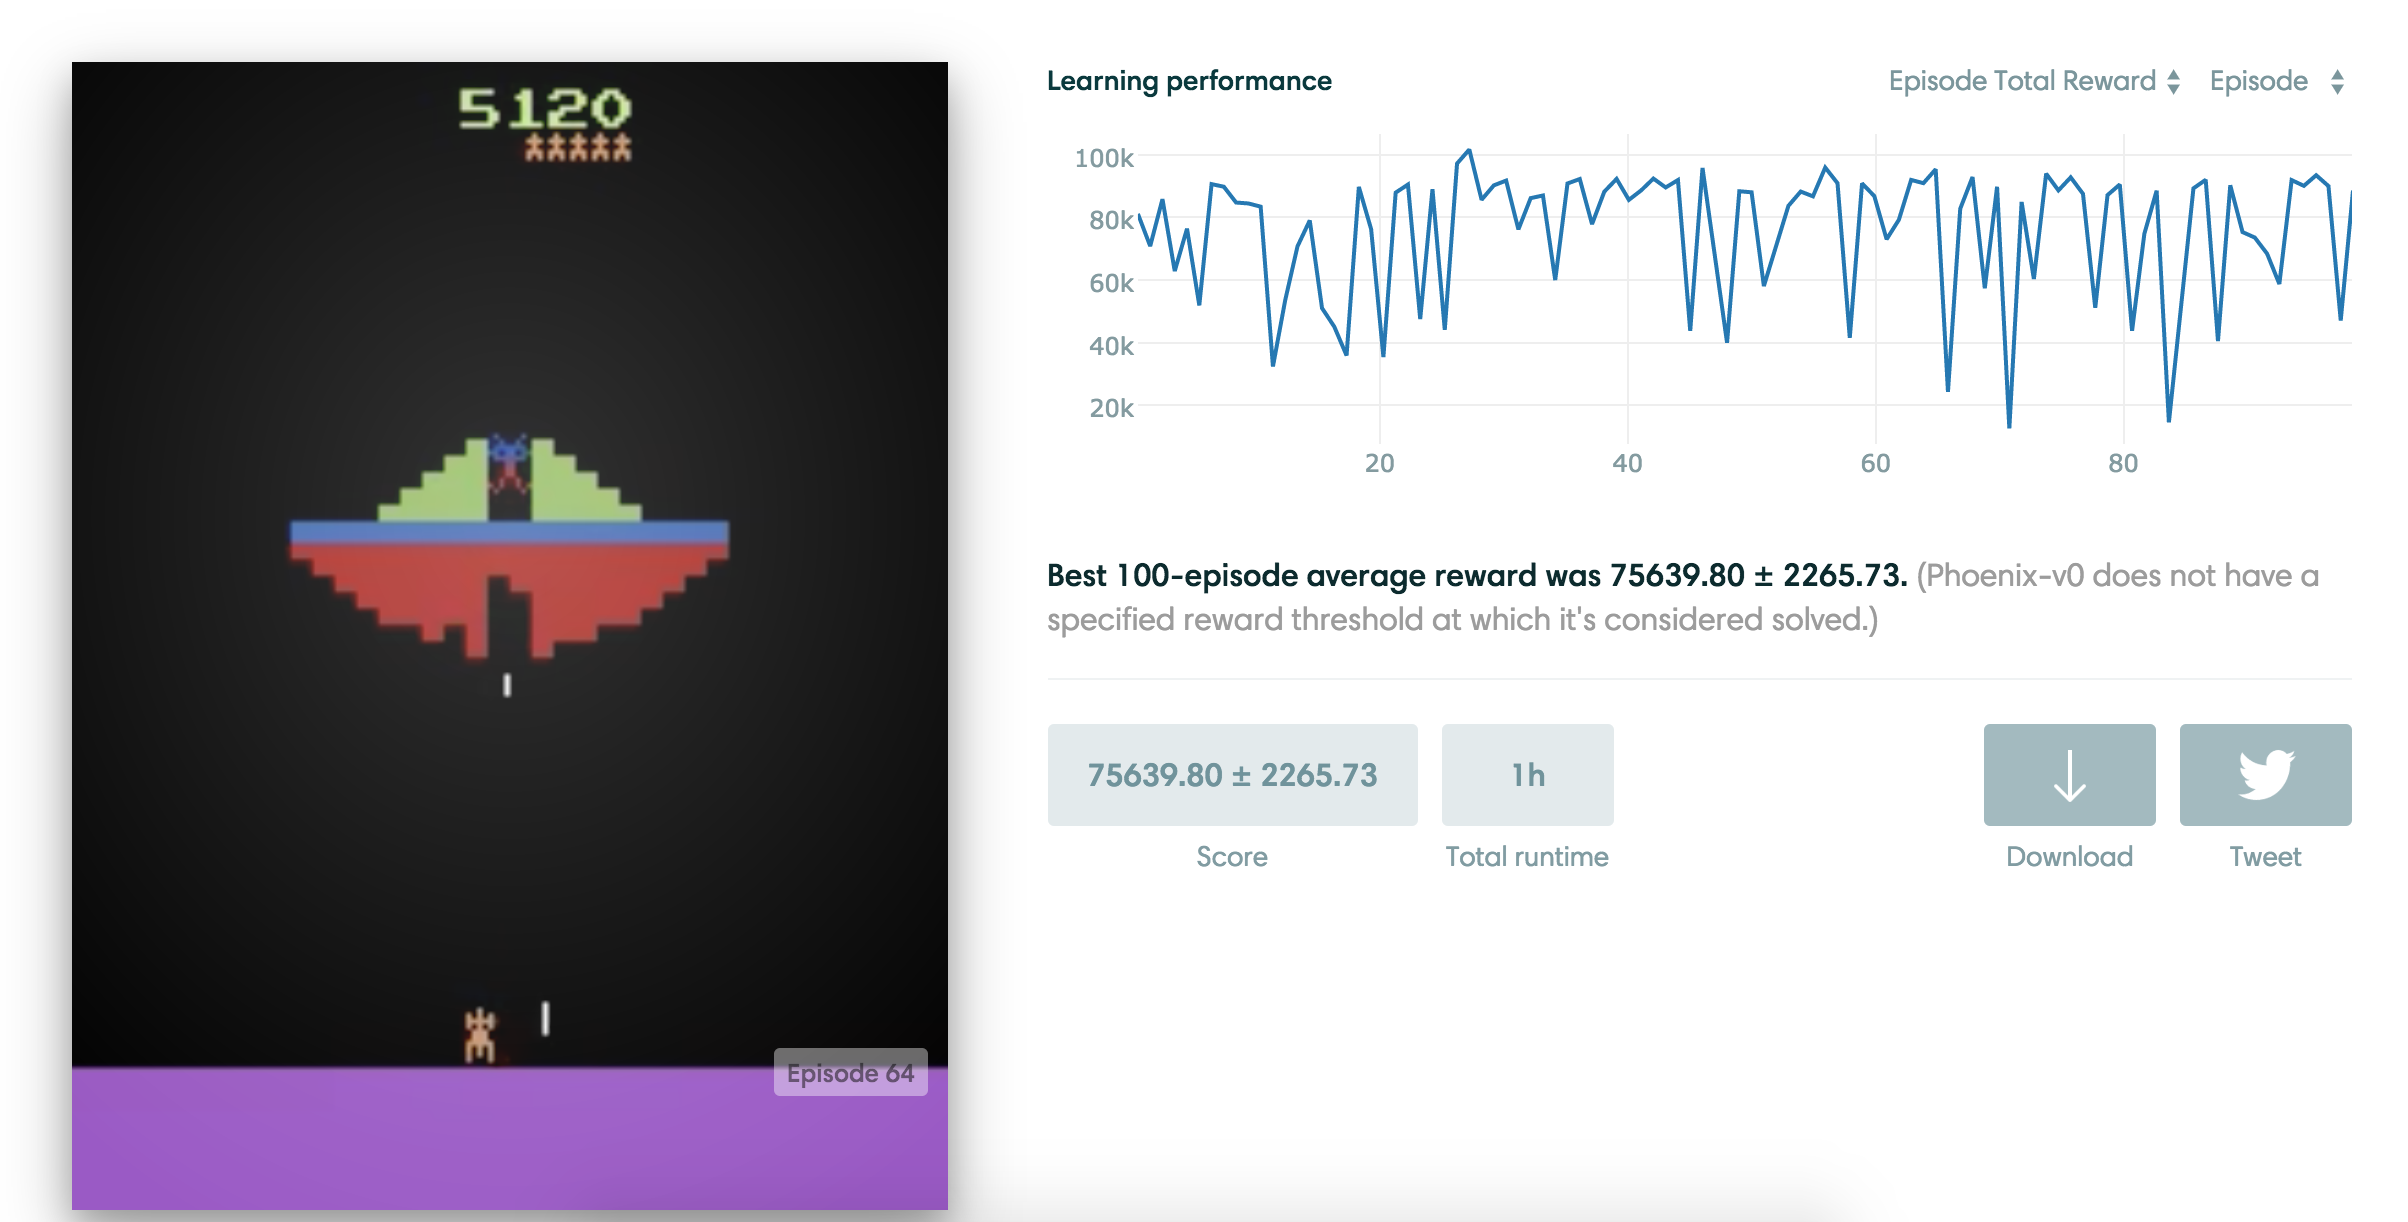
\includegraphics[width=0.49\textwidth]{./fig/A3C_Phoenix-v0.png} \\
(c) \href{https://gym.openai.com/evaluations/eval_Gva8XrEvTQi63KOd5Gyq1Q#reproducibility}{Phoenix-v0} \\
\end{tabular}
\caption{The results of 100 epsiodes on three environments by applying A3C algorithms. By clicking the name of each environment 
beneath the figures, you will see the video for each game played by trained agent.}
\label{fig:A3C_baselines}
\end{figure}







%-------------------------------------------------------------------------


\section{Time Line}
%!TEX root = main.tex


10/19-10/26: Review some related literatures about deep reinforcement learning-based games and related deep reinforcement learning methods. Figure out possible suitable methodologies and games to implement.

10/27-11/02: Review paper "Asynchronous Methods for Deep Reinforcement Learning". Learn to use OpenAI Gym, Keras software package.

11/09-11/16: Use Keras to define the deep q network. Write midterm paper.

11/16-11/23: OpenAI's gym library to interact with the game Learning Environment.

11/23-11/30: Use Tensorflow to optimization the network

12/01-12/13: Test the game. Write final report.





%-------------------------------------------------------------------------


{\small
\bibliographystyle{ieee}
\bibliography{egbib}
}

\end{document}
